\qitem{%
    An acute triangle $ABC$ is given with $BAC = 45^o$. Altitudes of this triangle intersect at point $H$. Prove that $| AH | = | BC |$.
    }{%
    $AH=2R\cos A$
    $BC=2R\sin A$
    Since $\sin 45^{\circ}=\cos 45^{\circ}$, $AH=BC$, as desired.
    }{%
    https://artofproblemsolving.com/community/c4t70430f4h2504818_ahbc_wanted_orthocenter__ltbac45o_acute_2006_polish_jmo_r2_p3
}

\qitem{%
    $AB,AC$ are tangents from $A$ to a circle touching the circle at $B,C$. If $D$ is the midpoint of the minor arc $BC$, prove that $D$ is the incentre of $\triangle ABC$
    }{%
    It is obvious that $\overline{AD}$ is the bisector of $\angle BAC$. Joining $\overline{DB}$ and $\overline{CD}$, we can tell that $\angle ABD = \angle ACD = \angle DBC = \angle DCB$. Thus, $\overline{BD}$ and $\overline{CD}$ are bisectors of $\angle ABC$ and $\angle ACB$, with them intersecting at $D$, which is the incenter of $\triangle ABC$.
    }{%
    https://artofproblemsolving.com/community/c3t120f3h1681395_circles_and_incentres
}

\qitem{%
    In triangle $ABC$, vertices $A$ and $C$, the center of the incircle and the center of the circumcircle lie on the same circle. Find $\angle B$.
    }{%
    If $O$ is the circumcenter and $I$ is the incenter
    $\angle AIC=180-\frac{1}{2}(\angle A+\angle C)=90+\frac{1}{2}\angle B$
    $\angle AOC=2\angle B$

    Since $AIOC$ is a cyclic quad, $\angle AIC=\angle AOC$, so $B=\frac{2}{3}(90)=\boxed{60}$
    }{%
    https://artofproblemsolving.com/community/c4t120f4h2329224_ltb_wanted_ac_oh_concyclic_oral_moscow_team_mo_2007_9a__p2
}

\qitem{%
    \myrightasy[2.2in]{
        Point $O$ is the circumcenter of triangle $ABC$, and point $A'$ is the reflection of point $A$ over line $BC$. Let $\omega$ be the circle passing through points $A$, $O$, and $A'$. Line $AB$ intersects $\omega$ at point $X$ different from $A$, and line $AC$ intersects $\omega$ at point $Y$ different from $A$. Prove that $\overline{YO} = \overline{XA'}$.
        }{
        import MOgeom;
        pair A, B, C, O, V, X, Y;
        A = (1, 4);
        V = (1, -4);
        B = (0, 0);
        C = (10, 0);
        O = circumcenter(A, B, C);
        path circleAOV;
        circleAOV = circumcircle(A, O, V);
        X = intersectionpoint(-A -- B, circleAOV);
        Y = intersectionpoint(A -- C, circleAOV);
        draw(X -- A -- C);
        draw(B -- C);
        draw(circleAOV);
        draw(Y -- O);
        draw(X -- V);
        dot(O);
        dot(V);
        label("$A$", A, N);
        label("$B$", B, W);
        label("$C$", C, E);
        label("$A'$", V, S);
        label("$O$", O, E);
        label("$X$", X, SSW);
        label("$Y$", Y, ENE);
    }
    }{%
    Let $D$ be the foot of the altitude from $A$ to $BC$. Notice that $\angle YAO = \angle CAO = 90^{\circ}-\angle B$ and $\angle XAA' = \angle BAD = 90^{\circ}-\angle B$, so $\angle YAO = \angle XAA'$. Thus, $YO=XA'$.
    }{%
    https://artofproblemsolving.com/community/c4t41805f4h2041554_nonsymmetrical_geometry_problem
}

\qitem{%
    Given a right-angled triangle $ABC$ with right angle $C$, $AA_1$ and $BB_1$ , it's angle bisectors. Points $A_2$ and $B_2$ are the feet of the perpendiculars drawn from $A_1$ and $B_1$ on $AB$. Prove that the center of the incircle of triangle $ABC$ coincides with the center of the circumcircle of triangle $A_2B_2C$.
    }{%
    Note that $\angle A_1CA=\angle A_1A_2A=90^0 \implies A_1A_2AC$ is cyclic. $\angle CAA_1=\angle A_1AA_2 \implies CA_1=A_1A_2$
    Also $\angle CA_1A+ \angle CAA_1=90^0 \implies \angle CA_1A+ \angle A_1CA_2=90^0 \implies A_1A \perp CA_2 \implies$ I is on the perpendicular bisector of $CA_2$. Analougsly, $I$ is also o the perpendicular bisector of $CB_2$.
    }{%
    https://artofproblemsolving.com/community/c4t120f4h2521468_incenter_of_abc_is_circumcenter_of_a_2b_2c_2021_aesc_msu_internet_olympiad_83
}

\qitem{%
    Let $ABC$ be an acute triangle with $AB >AC$ and $\angle BAC =60^o$. Denote the circumcenter by $O$ and orthocenter by $H$. The extension of $OH$ intersects $AB$ and $AC$ in $P$ and $Q$ respectively. Prove that $PO=HQ$.
    }{%
    $AH = 2R\cos 60^\circ = R = AO, \angle PAO=\angle QAH=90^\circ-\angle C, \angle AOP=\angle AHQ.$ Thus, triangles $APO, AQH$ are congruent and $PO=QH$.

    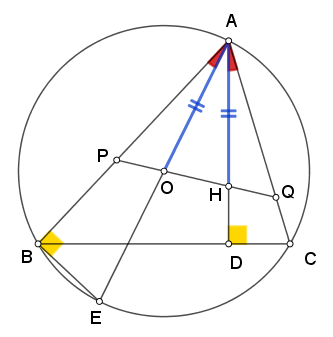
\includegraphics[width=0.3\linewidth]{../dgs2020/go5_pic/go5_ans_POequalHQ.png}
    }{%
    https://artofproblemsolving.com/community/c4t70430f4h1849571_equal_segments_orthocenter_and_circumcenter_related
}

\qitem{%
    Let $D$ be an interior point of the side $BC$ of a triangle $ABC$. Let $I_1$ and $I_2$ be the incentres of triangles $ABD$ and $ACD$ respectively. Let $AI_1$ and $AI_2$ meet $BC$ in $E$ and $F$ respectively. If $\angle BI_1E = 60^o$, what is the measure of $\angle CI_2F$ in degrees?
    }{%
    We have $\angle BI_1E=60^\circ$. So, $$\angle BAD=2\angle BAI_1=2(180^\circ-\angle B-\angle AEB) =2(180^\circ-\angle B-120^\circ+\frac{\angle B}{2})=120^\circ-\angle B$$Now, $\angle CAD=\angle A-(120^\circ-\angle B) =-120^\circ+180^\circ-\angle C=60^\circ-\angle C$. With similar calculations like for $\angle BI_2E\rightarrow \angle BAD$ we have $$\angle CI_2F=\boxed{30^\circ}$$
    }{%
    https://artofproblemsolving.com/community/c4t120f4h1891374_2018_prermo_p29_angle_chasing_candidate_2_incentres_given
}

\qitem{%
    Let $ABC$ be a triangle with$\angle B > \angle C$. The angle bisector of $\angle A$ intersects $BC$ at $D$. The perpendicular from $B$ to $AD$ intersects the circumcircle of $\triangle ABD$ again at $E$. Prove that the circumcenter of $\triangle ABC$ lies on the line $AE$.
    }{%
    \myrightasy[2.5in]{
        Let the circumcenter of $\triangle ABC$ be $O$. We have
        $$\angle OAB=\tfrac12(180^\circ-\angle AOB)=\tfrac12(180^\circ-2\angle ACB)=90^\circ-\angle ACB$$Also, we have:
        $$\angle EBA=90^\circ-\angle BAD =90^\circ-\tfrac12\angle BAC$$and
        $$\angle AEB=\angle ADB=180^\circ-\angle BAD-\angle ABC=180^\circ-\tfrac12\angle BAC-\angle ABC$$Therefore,
        \begin{align*} \angle EAB&=180^\circ-\angle EBA-\angle AEB\\ &=180^\circ-(90^\circ-\tfrac12\angle BAC)-(180^\circ-\tfrac12\angle BAC-\angle ABC)\\ &=\angle BAC+\angle ABC-90^\circ\\ &=(180^\circ-\angle ACB)-90^\circ\\ &=90^\circ-\angle ACB\\ &=\angle OAB \end{align*}Therefore, $A,E,O$ all lie on the same line.
        }{
        import MOgeom;
        size(2inch);
        pair A=(0,2),B=(-1,0),C=(2,0);
        pair D = intersectionpoint(B--C,A--(A+(bisectorpoint(B,A,C)-A)*3));
        pair E = intersectionpoint(circumcircle(A,B,D),foot(B,A,D)--(B+(foot(B,A,D)-B)*3));
        draw(A--B--C--cycle);
        draw(circumcircle(A,B,D));
        draw(A--D);draw(B--E--A);
        dot(circumcenter(A,B,C));
        label("$O$",circumcenter(A,B,C),dir(50));
        label("$E$",E,dir(-20));
        label("$A$",A,dir(75));
        label("$D$",D,dir(-60));
        label("$B$",B,SW);
        label("$C$",C,SE);
    }
    }{%
    https://artofproblemsolving.com/community/c4t41805f4h1847981_position_of_circumcenter
}

